\documentclass[preprint,12pt]{elsarticle}
\usepackage{amsmath,amssymb,amsthm,booktabs,graphicx,xcolor}
\usepackage{xr-hyper}
\usepackage[hidelinks]{hyperref}
\externaldocument[][nocite]{sod_rom_v5_supp}
\usepackage{tikz}
\usepackage[subpreambles=true]{standalone}  % Fig. 1 is the TikZ file ../figures/tikz/fig_c_systems_tikz.tex
% shared macros for the SOD tutorial and papers
% Typesetting follows ISO 80000-2: italic scalars (capital Greek via \var...),
% bold italic vectors and matrices (\bm), upright d, e, i, operators and labels.
\usepackage{bm,upgreek}
\newcommand{\bx}{\bm{x}}  \newcommand{\bz}{\bm{z}}  \newcommand{\bX}{\bm{X}}
\newcommand{\bV}{\bm{V}}  \newcommand{\bW}{\bm{W}}  \newcommand{\bU}{\bm{U}}
\newcommand{\bM}{\bm{M}}  \newcommand{\bK}{\bm{K}}  \newcommand{\bC}{\bm{C}}
\newcommand{\bA}{\bm{A}}  \newcommand{\bB}{\bm{B}}  \newcommand{\bS}{\bm{S}}
\newcommand{\bI}{\bm{I}}  \newcommand{\bff}{\bm{f}}
\newcommand{\bSig}{\bm{\varSigma}}  \newcommand{\bpsi}{\bm{\psi}}  \newcommand{\bPsi}{\bm{\varPsi}}
\newcommand{\bphi}{\bm{\phi}}  \newcommand{\bPhi}{\bm{\varPhi}}
\newcommand{\avg}[1]{\left\langle #1 \right\rangle}
\newcommand{\bnd}[1]{\left[ #1 \right]_T}
\newcommand{\sym}{\operatorname{sym}}  \newcommand{\skw}{\operatorname{skew}}
\newcommand{\TODO}[2]{\textcolor{red}{\textbf{[#1]} #2}}

% scalars: A, E, H, I, L, P, R, T, W, \varOmega, \varGamma
% elsarticle appends a period to every \paragraph title; the titles here carry
% their own punctuation (some end in '?'), so the automatic period is removed.
\makeatletter
\def\els@aparagraph[#1]#2{\elsparagraph[#1]{#2}}
\def\els@bparagraph#1{\elsparagraph*{#1}}
\makeatother
\graphicspath{{../figures/}}
\newtheorem{proposition}{Proposition}
\setlength{\emergencystretch}{3em}
\journal{Journal of Sound and Vibration}
\begin{document}
\begin{frontmatter}
\title{What a free decay teaches a smooth orthogonal decomposition basis}
\author[nld]{David Chelidze}
\ead{chelidze@uri.edu}
\affiliation[nld]{organization={Nonlinear Dynamics Laboratory, Department of Mechanical, Industrial and Systems Engineering, University of Rhode Island},
            city={Kingston}, state={RI}, postcode={02881}, country={USA}}


\begin{abstract}
Smooth orthogonal decomposition (SOD) builds reduced-order model (ROM) bases from response records. Trained on one free decay, it gives three different outcomes.
On a Rayleigh-damped cantilever the basis is the linear normal modes (LNMs), within 12\,\% in ROM error.
With a tip dashpot it is 6 times more accurate than the LNMs at eight modes and 3.5--6 times less accurate at two to five.
With a cubic tip spring it lowers the backbone error by two to three decades.
We test one explanation. A free decay is driven only by internal forces, and the SOD basis holds the modes plus, for a force concentrated at one point, the structure's response to a force there at the direction's own SOD frequency.
A covariance identity, which keeps the force term of the SOD eigenproblem, states this with its damping and record-end corrections.
The dashpot decay has one non-modal direction, $17^\circ$ from the nearest LNM and $2.5^\circ$ from the tip-force response. On two nonlinear cantilevers the first SOD direction lies within $0.05^\circ$ of that response.
The obstacle is ranking: SOD orders that direction among the modes by its frequency, and at low order it displaces a mode.
Modal planes recognised by their one-way rotation in the displacement--velocity state mark the modal directions; with these placed first, the decay basis equalled the LNMs at two to five modes and kept its gain from six, for both dashpots tested.
Its ROM errors then track modal truncation augmentation with the tip static vector, which must be told where the force acts; the decay was not.
Forced training records are used only as a contrast. All results are numerical, from full-field records with model velocities.
\end{abstract}

\begin{keyword}
smooth orthogonal decomposition \sep reduced-order model \sep free decay \sep static correction \sep modal truncation augmentation \sep mode recognition \sep nonlinear normal mode
\end{keyword}
\end{frontmatter}

\section{Introduction}\label{sec:intro}
Projection-based reduced-order models (ROMs) replace $n$ physical coordinates by $r\ll n$ generalized coordinates.
For linear structures the classical basis is the set of linear normal modes (LNMs).
Truncated modes still respond quasi-statically to the load. Static correction, or modal truncation augmentation (MTA), adds that response to the basis as the static deflection under the part of each load that the retained modes miss \citep{Dickens1997}. The mode-acceleration method adds the same term after the modal solution \citep{Cornwell1983}.
Load-dependent Ritz vectors build the whole basis from the load: the first is its static deflection, and each next one is the static response to the inertia load of the last \citep{Wilson1982}.
Input-aware reduction is also standard in systems and control, through balanced truncation \citep{Moore1981} and Krylov moment matching \citep{Bai2002}. \citet{Besselink2013} compared these methods with modal reduction on a structural model.
All of them need the model and the load locations.
Data-driven bases are built from response records, without an eigensolution of the model. Proper orthogonal decomposition (POD) is the common choice \citep{Kerschen2005}. Its modes equal the normal modes only in special cases, such as free vibration with a mass matrix proportional to the identity \citep{Feeny1998}.
Smooth orthogonal decomposition (SOD) solves the generalized eigenproblem of the displacement and velocity covariances \citep{Chelidze2006,Farooq2008}. For undamped free vibration it returns the LNMs and the natural frequencies, with no mass matrix.
SOD subspaces have served as ROM bases for nonlinear systems \citep{Segala2015,Ilbeigi2017,Ilbeigi2018}; \citet{Ilbeigi2017} reported that SOD outperformed POD in stability, accuracy and robustness.
These studies did not identify which directions a data basis contains that the normal modes lack.

Free decays make the question sharp, because a decay has no external load to learn from. We trained SOD on one band-limited free decay of a cantilever and tested the ROM under random loads.
With Rayleigh damping the decay basis gave the LNM errors, within 12\,\% at every order to eight.
With a dashpot from the tip to ground, the same construction was 6 times more accurate than the LNMs at eight modes ($1.9\times10^{-5}$ against $1.1\times10^{-4}$) and 3.5--6.3 times less accurate at two to five.
With a cubic spring at the tip, a decay-trained basis lowered the backbone error of the first nonlinear normal mode (NNM) by two to three decades.
A basis that is the modes, better than the modes and worse than the modes is not explained by saying that SOD approximates the LNMs.

This paper tests one explanation. In a free decay the only forces are internal. Distributed proportional damping leaves the modes uncoupled, and SOD returns them. A dashpot, a magnet or a nonlinear spring is a force concentrated at one point. The decay then contains the structure's response to a force at that point, and SOD returns it as one more direction: the response at that direction's own SOD frequency. Its low-frequency limit is the static vector that MTA adds when told the location. This is a hypothesis to be tested, not an established cause.

It can be stated exactly. \citet{Farooq2008} wrote the SOD eigenproblem of a forced undamped system with the force--response covariance kept, and showed that the term vanishes for white-noise excitation, which leaves the structural eigenproblem. We keep the term, with the internal force as the input, and add the damping and record-end terms (Section~\ref{sec:identity}).

Acting on the explanation is not straightforward, because of how SOD ranks directions. It orders them by mean-square frequency. The force-response direction has a frequency of its own, which falls among the modes, and in a truncated basis it displaces one of them.
The idea that removes the obstacle is to recognise each direction by what it does, not by its rank. A modal plane of SOD applied to the displacement--velocity state rotates one way. The planes so recognised mark the modal directions of the configuration basis, which are placed first; the force-response direction follows.


SOD has relatives that sharpen what is specific to it.
The same pencil, with first differences, appeared earlier in statistics as maximum autocorrelation factors \citep{Switzer1984,Shapiro1989}. It is also linear slow feature analysis \citep{Wiskott2002}. Lagged second-order statistics underlie the blind-separation methods AMUSE (algorithm for multiple unknown signals extraction) and SOBI (second-order blind identification) \citep{Tong1991,Belouchrani1997}. Related smooth decompositions were studied by \citet{Bellizzi2009,Bellizzi2012}.
\citet{Feeny2008} decomposed the state with a non-symmetric pencil that returns complex modes; \citet{Farooq2012} tested it on experimental data. Our state-space SOD keeps the symmetric pencil instead.
The spatial dual of SOD, smooth mode decomposition (SMD), smooths the mode shapes in space rather than the coordinates in time \citep{Li2023}. SOD has been placed among other data-driven modal decompositions as a characteristic value decomposition \citep{Li2025}, and bases of that kind have served nonlinear normal mode (NNM) continuation with ROMs \citep{Stein2025}. \citet{Khan2020} related POD and SOD to the state-variable and dynamic mode decompositions \citep{Schmid2010}.
Identification of frequencies and damping from measured records, with estimated kinematics, is outside this paper.

Sections~\ref{sec:method} and \ref{sec:bench} give the method, the identity and the benchmarks. Section~\ref{sec:puzzle} shows the puzzle in the data. Section~\ref{sec:decayadds} tests what the decay adds, and Section~\ref{sec:order} locates and removes the low-order loss. Section~\ref{sec:nonlin} applies the explanation to two nonlinear cantilevers. Section~\ref{sec:contrast} contrasts forced training records and heavy proportional damping. Section~\ref{sec:disc} weighs the evidence. The supplementary material holds the forced-record study, the complex-mode study, integration cost and detailed variants; its sections, figures and tables carry the prefix S.


\section{Method}\label{sec:method}
\subsection{Galerkin ROMs and bases}
The full model is $\bM\ddot\bx+\bC\dot\bx+\bK\bx=\bm{B}\bm{u}(t)$. Here $\bM$, $\bC$ and $\bK$ are the mass, damping and stiffness matrices, $\bx$ is the displacement, and $\bm{B}$ distributes the $m$ load inputs $\bm{u}(t)$.
With $\bx\approx\bm{\varPhi}\bm{q}$, generalized coordinates $\bm{q}$ and a basis $\bm{\varPhi}\in\mathbb{R}^{n\times r}$ of full column rank, Galerkin projection gives
\begin{equation}
\bm{\varPhi}^{\mathsf T}\bM\bm{\varPhi}\,\ddot{\bm{q}}+\bm{\varPhi}^{\mathsf T}\bC\bm{\varPhi}\,\dot{\bm{q}}+\bm{\varPhi}^{\mathsf T}\bK\bm{\varPhi}\,\bm{q}=\bm{\varPhi}^{\mathsf T}\bm{B}\bm{u}.
\label{eq:rom}
\end{equation}
The reduced matrices inherit symmetry and definiteness. Every such ROM is therefore non-expansive in the energy norm when $\bM,\bK\succ0$ and $\bC\succeq0$.
Initial states are projected $\bM$-orthogonally, $\bm{q}_0=(\bm{\varPhi}^{\mathsf T}\bM\bm{\varPhi})^{-1}\bm{\varPhi}^{\mathsf T}\bM\bx_0$.
Configuration bases:
\begin{itemize}
\item \emph{LNM}: the $r$ lowest undamped modes of $(\bK,\bM)$;
\item \emph{MTA}: the $r-m$ lowest LNMs plus the $m$ static load vectors $\bK^{-1}\bm{B}$, $\bM$-orthonormalized, which spans the same subspace as the modal truncation vectors of \citet{Dickens1997};
\item \emph{POD}: the $r$ leading eigenvectors of $\bSig_x=\avg{\bx\bx^{\mathsf T}}$;
\item \emph{SOD}: the $r$ smoothest smooth modes $\bphi_i=\bSig_x\bpsi_i$, where $\bSig_v=\avg{\dot\bx\dot\bx^{\mathsf T}}$ and $\bSig_v\bpsi=\mu\bSig_x\bpsi$ with $\mu$ ascending and $\bpsi_i^{\mathsf T}\bSig_x\bpsi_i=1$. The values $\mu$ are the smooth orthogonal values (SOVs). For full-rank data the smooth modes are the columns of $\bPsi^{-\mathsf T}$. Here SOD is the temporal form, and a smooth mode is the shape paired with a temporally smooth coordinate, not a spatially smoothed shape as in SMD.
\end{itemize}
MTA-tip denotes MTA with the tip vector $\bK^{-1}\bm{e}_{\mathrm{tip}}$ only, where $\bm{e}_{\mathrm{tip}}$ is the unit load at the tip displacement; it is told where the dashpot or the nonlinear spring acts.
Band-limited records leave $\bSig_x$ nearly singular. SOD is solved in the POD subspace whose eigenvalues exceed $10^{-10}$ of the largest. Section~\ref{sec:rank} varies this tolerance.
Data-driven bases stop at that data rank. No ROM is reported at an order the basis cannot supply.
At the data rank, SOD and POD span the same subspace. A Galerkin ROM depends only on the subspace, so their ROMs coincide there.

\subsection{State-space SOD for complex modes}\label{sec:ssod}
Non-proportional damping makes the modes complex. Configuration SOD returns real vectors and cannot represent them.
We then apply SOD to the state $\bm{y}=(\bx,\dot\bx)$, with state matrix $\bm{A}$, input matrix $\bm{B}_{\mathrm s}$ and $\dot{\bm{y}}=\bm{A}\bm{y}+\bm{B}_{\mathrm s}\bm{u}$:
\begin{equation}
\avg{\dot{\bm{y}}\dot{\bm{y}}^{\mathsf T}}\bpsi=\mu\,\avg{\bm{y}\bm{y}^{\mathsf T}}\bpsi.
\label{eq:ssod}
\end{equation}
The pencil stays real and symmetric. It is invariant under any linear change of state coordinates, so mixing displacement and velocity units is harmless.
In real modal coordinates, $\bm{y}=\bm{P}\bm{\xi}$ with $\bm{P}_i=(\operatorname{Re}\,\bm{v}_i,\operatorname{Im}\,\bm{v}_i)$, each complex eigenvalue pair $s_i=\sigma_i+\mathrm i\omega_i$ of $\bm{A}$, with eigenvector $\bm{v}_i$, owns a plane with $\dot{\bm{\xi}}_i=\bm{L}_i\bm{\xi}_i$, $\bm{L}_i=\big[\begin{smallmatrix}\sigma_i&\omega_i\\-\omega_i&\sigma_i\end{smallmatrix}\big]$ and $\det\bm{L}_i=|s_i|^2$.

\begin{proposition}[State-space SOD]\label{prop:ssod}
Let the response be free and the modal planes uncorrelated, $\avg{\bm{\xi}\bm{\xi}^{\mathsf T}}=\operatorname{blockdiag}(\bm{G}_i)$. Then each plane contributes two values with $\mu_{i,a}\mu_{i,b}=|s_i|^4$. Its two smooth modes span the modal plane $(\operatorname{Re}\,\bm{v}_i,\operatorname{Im}\,\bm{v}_i)$. The two values are equal if and only if $\bm{G}_i\propto\bm{I}$.
\end{proposition}
\noindent \ref{app:proofs} gives the proof. In brief, the pencil decouples by plane, and $\det(\bm{L}_i\bm{G}_i\bm{L}_i^{\mathsf T})/\det\bm{G}_i=|s_i|^4$.
For an undamped mode, isotropy of $\bm{G}_i$ is the modal virial balance. The pair product needs only decorrelation.

Two ROM constructions are natural.
\begin{itemize}
\item \emph{Petrov--Galerkin} with the data covectors: $\bm{q}=\bm{\varPsi}^{\mathsf T}\bm{y}$, $\dot{\bm{q}}=\bm{\varPsi}^{\mathsf T}\bm{A}\bm{\varPhi}\bm{q}+\bm{\varPsi}^{\mathsf T}\bm{B}_{\mathrm s}\bm{u}$.
\item \emph{Energy Galerkin} on the smooth-mode subspace, with test basis $\bm{W}\bm{\varPhi}$ and $\bm{W}=\operatorname{blockdiag}(\bK,\bM)$.
\end{itemize}
The first failed: data covectors are undetermined outside the span of the data, and their input coupling $\|\bm{\psi}_i^{\mathsf T}\bm{B}_{\mathrm s}\|$ reached $2\times10^3$--$3\times10^5$ (Section~\ref{sec:s-pg}).
The second inherits stability. For $\bM,\bK\succ0$ and symmetric $\bC\succeq0$, $\bm{W}\bm{A}+\bm{A}^{\mathsf T}\bm{W}=\operatorname{blockdiag}(\mathbf 0,-2\bC)\preceq0$. With $\bm{E}=\bm{\varPhi}^{\mathsf T}\bm{W}\bm{\varPhi}$ and $\bm{A}_r=\bm{E}^{-1}\bm{\varPhi}^{\mathsf T}\bm{W}\bm{A}\bm{\varPhi}$, the same holds for $\bm{E}\bm{A}_r+\bm{A}_r^{\mathsf T}\bm{E}$, so the ROM is non-expansive in the energy norm. On S3 (below) with tip-dashpot coefficient $c_{\mathrm d}=0.2$, a free-decay basis and a random load, its errors were $0.16$, $4.1\times10^{-2}$, $1.3\times10^{-2}$, $4.5\times10^{-3}$ for state dimension 2 to 8. We use it throughout.
The model-based counterpart is complex-mode truncation (CM): the slowest eigen-planes of $\bm{A}$, projected with the left eigenvectors.
State ROMs are compared with configuration ROMs at equal state dimension, $2r$.

\subsection{What a record adds: a covariance identity}\label{sec:identity}
Let one force history $f(t)$ act through the vector $\bm{b}$: $\bM\ddot\bx+\bC\dot\bx+\bK\bx=\bm{b}f(t)$. The force may be an external load. In a free decay it is an internal force taken to the right-hand side: a dashpot force $-c_{\mathrm d}\dot x_{\mathrm{tip}}$, or a nonlinear spring force; $\bC$ and $\bK$ then hold the rest of the model. Write $[\bm{g}]_0^T=\bm{g}(T)-\bm{g}(0)$ for a record of length $T$.

\begin{proposition}[Covariance identity]\label{prop:identity}
Let $(\mu_i,\bpsi_i)$ be an SOD pair of the record, with full-rank data, and $\bphi_i=\bSig_x\bpsi_i$ its smooth mode. Then
\begin{equation}
(\bK-\mu_i\bM)\,\bphi_i=\bm{b}\,\avg{f\bx^{\mathsf T}}\bpsi_i-\bC\avg{\dot\bx\bx^{\mathsf T}}\bpsi_i-\frac1T\,\bM\big[\dot\bx\bx^{\mathsf T}\big]_0^T\bpsi_i .
\label{eq:identity}
\end{equation}
\end{proposition}
\noindent\emph{Proof.} Multiply the equation of motion on the right by $\bx^{\mathsf T}$ and average over the record: $\bM\avg{\ddot\bx\bx^{\mathsf T}}+\bC\avg{\dot\bx\bx^{\mathsf T}}+\bK\bSig_x=\bm{b}\avg{f\bx^{\mathsf T}}$. Integration by parts gives $\avg{\ddot\bx\bx^{\mathsf T}}=[\dot\bx\bx^{\mathsf T}]_0^T/T-\bSig_v$. Apply the result to $\bpsi_i$ and use $\bSig_v\bpsi_i=\mu_i\bSig_x\bpsi_i$. \hfill$\square$

The undamped form with the force term, for long records, is Eq.~(8) of \citet{Farooq2008}. Three readings follow.
\begin{itemize}
\item \emph{No concentrated force.} With $f=0$, no damping and a record whose end term vanishes, $(\bK-\mu_i\bM)\bphi_i=\mathbf 0$: the smooth modes are the LNMs and $\mu_i=\omega_i^2$ \citep{Chelidze2006}. Proportional damping perturbs this through the second term.
\item \emph{One concentrated force.} The first term is the vector $\bm{b}$ times a scalar. Where it dominates, $\bphi_i$ is parallel to
\begin{equation}
\bm{d}(\omega)=(\bK-\omega^2\bM)^{-1}\bm{b}\quad\text{at}\quad\omega=\sqrt{\mu_i},
\label{eq:d}
\end{equation}
the undamped response of the structure to a harmonic force at that point. At $\omega=0$ it is the static vector $\bK^{-1}\bm{b}$ of MTA. For a mode, the scalar $\avg{f\bx^{\mathsf T}}\bpsi_i$ and the factor $\bK-\mu_i\bM$ are both small, and $\bm{d}$ at a frequency near $\omega_k$ is nearly LNM~$k$.
\item \emph{Record ends.} The last term vanishes for a decay released from rest and recorded until it has died out.
\end{itemize}
SOD solved in the POD subspace of Section~\ref{sec:method} adds a rank term, $\bM(\bSig_v-\mu_i\bSig_x)\bpsi_i$. With sampled covariances the terms closed to $10^{-11}$ of $\|\bphi_i\|_{\bM}$ or better in every record used here (\texttt{i1\_forced\_identity.py}).


\subsection{What to expect}\label{sec:expect}
Write $\bx=\bPhi\bm{\eta}$ with mass-normalized LNMs, and $\bm{G}_x=\avg{\bm{\eta}\bm{\eta}^{\mathsf T}}$, $\bm{G}_v=\avg{\dot{\bm{\eta}}\dot{\bm{\eta}}^{\mathsf T}}$.
Configuration SOD returns the LNMs if and only if $\bm{G}_x$ and $\bm{G}_v$ are diagonal. It returns the frequencies $\omega_i$ if also $(\bm{G}_v)_{ii}=\omega_i^2(\bm{G}_x)_{ii}$ (\ref{app:proofs}).
Modal correlation rotates the modes at first order. A virial defect $\delta_i$, defined by $(\bm{G}_v)_{ii}=\omega_i^2(1+\delta_i)(\bm{G}_x)_{ii}$, shifts the frequency by $\delta_i/2$ but leaves the modes alone.
For a single-degree-of-freedom decay from rest with damping ratio $\zeta$, the defect is $-4\zeta^2/(1+4\zeta^2)$, so the frequency bias is second order in damping. A nonzero initial velocity adds a first-order term that averages out over phase.
Free decay under proportional damping nearly satisfies both conditions. Forced response does not:
\begin{itemize}
\item single-point forcing correlates the modal coordinates;
\item modes above the load band respond quasi-statically, at the load frequencies.
\end{itemize}
SOD ranks motions by smoothness, POD by variance. A quasi-static direction can therefore enter either basis early.

\subsection{Geometric measures of a basis}\label{sec:geommeasure}
A Galerkin ROM depends only on the subspace its basis spans. Two measures compare subspaces directly.
For a basis $\bm{\varPhi}_r$ of $r$ columns, let $\bm{P}_r=\bm{\varPhi}_r(\bm{\varPhi}_r^{\mathsf T}\bM\bm{\varPhi}_r)^{-1}\bm{\varPhi}_r^{\mathsf T}\bM$ be the $\bM$-orthogonal projector onto its span. The containment residual of a vector $\bm{s}$ is
\begin{equation}
\rho_r(\bm{s})=\frac{\|(\bI-\bm{P}_r)\bm{s}\|_{\bM}}{\|\bm{s}\|_{\bM}},\qquad \|\bm{s}\|_{\bM}^2=\bm{s}^{\mathsf T}\bM\bm{s}.
\label{eq:contain}
\end{equation}
It is zero when $\bm{s}$ lies in the span and one when $\bm{s}$ is $\bM$-orthogonal to it. The static load vectors $\bK^{-1}\bm{b}$, with $\bm{b}$ a column of $\bm{B}$, are the directions MTA adds.
Two subspaces of equal dimension are compared by their principal angles in the $\bM$ inner product. The largest angle is zero only when the subspaces coincide.

\section{Benchmarks}\label{sec:bench}
Figure~\ref{fig:systems} shows the five systems. S1--S3 are linear and nondimensional; S4 is nonlinear and dimensional; S5 is nonlinear and nondimensional.
\begin{itemize}
\item \emph{S1, shear frame.} Ten stories, unit masses $m_j$, story stiffnesses $k_{\mathrm s,j}$ tapering linearly to 55\,\% at the top. Base acceleration input $\ddot x_{\mathrm g}$. $\omega_1,\dots,\omega_6=2.74$, $7.67$, $12.5$, $17.1$, $21.3$, $24.9$; $\omega_{\max}=36.2$.
\item \emph{S2, cantilever.} Thirty Euler--Bernoulli Hermite elements, consistent mass. Bending stiffness $EI$, mass per unit length $m'$ and length $L$ are $EI=m'=L=1$; $n=60$. Tip and mid-span forces $f_{\mathrm{tip}}$ and $f_{\mathrm{mid}}$. $\omega_1,\dots,\omega_5=3.52$, $22.0$, $61.7$, $121$, $200$; $\omega_{\max}=5.4\times10^4$.
\item \emph{S3, cantilever with tip dashpot.} S2 plus a viscous dashpot from the tip to ground, $c_{\mathrm d}=0.2$ or $1$.
\item \emph{S4, nonlinear cantilever.} The COST F3 benchmark \citep[Sec.~4.4, Table~1]{Peeters2009}: a steel beam, $L=0.7$\,m, $14\times14$\,mm, 20 elements. A cubic spring, $k_3=6\times10^9$\,N/m$^3$, runs from the tip to ground. Its first linear frequency is 23.66\,Hz. It is trained on damped decays released from static tip deflections (Section~\ref{sec:nlbb}).
\item \emph{S5, two-well cantilever.} A ten-element cantilever with a two-well tip force, under harmonic base acceleration. It is trained on one cross-well decay (Section~\ref{sec:moon}).
\end{itemize}
Damping cases:
\begin{itemize}
\item light Rayleigh, $\zeta=0.02$ at modes 1 and 4;
\item heavy Rayleigh, $\zeta=0.20$ at modes 1 and 4 (0.48 at mode 6 of S2);
\item non-proportional: light Rayleigh plus the dashpot. $c_{\mathrm d}=0.2$ gives $\zeta_1=0.13$ and $c_{\mathrm d}=1$ gives $\zeta_1=0.60$.
\end{itemize}
Rayleigh damping keeps the modes real \citep{Caughey1965}, so S1 and S2 use configuration SOD. S3 has complex modes. Its ROM bases here are configuration SOD bases; state-space SOD serves to recognise the modal planes (Section~\ref{sec:order}).

\begin{figure}[tbp]
\centering
\includestandalone[width=\textwidth,mode=tex]{../figures/tikz/fig_c_systems_tikz}
\caption{Benchmarks. (a) Ten-story shear frame under base acceleration. (b) Finite-element cantilever with tip and mid-span loads. (c) The same cantilever with a tip dashpot to ground. (d) COST F3 cantilever with a cubic spring from the tip to ground, released from a static tip load $P$. (e) Two-well cantilever under base acceleration $A\cos\varOmega t$: buckled equilibria $\pm x^*$ (exaggerated) and the double-well potential of the tip force.}
\label{fig:systems}
\end{figure}

\paragraph{Training and testing.} The bases of the main text were trained on free decays. Random and swept-sine records serve the contrast of Section~\ref{sec:contrast} and the supplement. Each record covers about 100 periods of mode 1:
\begin{itemize}
\item random: band-limited white noise to $\omega_{\mathrm c}$, at the base (S1) or the tip (S2, S3);
\item free decay, released from rest. The main decay (BL) has band-limited equal energy matched to the ROM order. Static release (SR) serves for contrast. Initial states are given below;
\item swept sine from $\omega_0$ to $\omega_{\mathrm c}$ at the same input.
\end{itemize}
Here $\omega_{\mathrm c}=23$ (S1) and 250 (S2, S3) cover five modes.
Tests used a new random load at the training input and a random load at mid-span (S2, S3). Two test decays followed. The first was an SR decay from another static load. The second was a BL decay band-limited at $\omega_{\mathrm c}$, with alternating signs.
Each of 20 realizations drew new random training and test loads.
Responses were computed exactly for piecewise-constant input.
The error is $\|\bX_r-\bX\|_{\bM}/\|\bX\|_{\bM}$ over the record. Here $\bX$ and $\bX_r$ hold the full-model and ROM displacements $\bx_k$ at the samples $k$, with $\|\bX\|_{\bM}^2=\sum_k\bx_k^{\mathsf T}\bM\bx_k$, so translations and rotations are weighted consistently.
Training velocities, and the accelerations of state-space SOD, come from the model. For model reduction the training records come from the model, so their velocities and accelerations are exact.

\paragraph{Initial states.} All decays start from rest at $\bx_0$, scaled so that its largest entry is 1. The scale does not affect relative errors of a linear model.
\begin{itemize}
\item \emph{Static release (SR)}: $\bx_0\propto\bK^{-1}\bm{f}$. Training: $\bm{f}=\bM\mathbf 1$ (unit force per floor, S1); unit tip force plus 0.7 at mid-span (S2, S3). Test: unit force at floor 4 (S1); 0.3 at the tip plus 1 at mid-span (S2, S3).
\item \emph{Equal energy (EE)}: $\bx_0\propto\sum_k b_k\bPhi\bm{e}_k/\omega_k$. Here $\bPhi\bm{e}_k$ is the $k$th mass-normalized LNM, with $\bm{e}_k$ the $k$th unit vector. Each mode then holds the same energy at $t=0$. The sum runs over all modes with $\omega_k<\uppi/(4\Delta t)$, for time step $\Delta t$: all ten for S1, modes 1--9 for the beams. Training uses signs $b_k=1$; the test uses $b_k=(-1)^{k-1}$.
\item \emph{Band-limited equal energy (BL)}: EE with $b_k$ multiplied by $a_k=1/[1+(\omega_k/\omega_{\mathrm b})^4]$. Modes below $\omega_{\mathrm b}$ hold nearly equal energy; above it the energy falls as $(\omega_{\mathrm b}/\omega_k)^8$. The main training decay uses $\omega_{\mathrm b}=\omega_r$, the frequency of LNM~$r$. Each ROM order thus has its own decay. The BL test decay uses $\omega_{\mathrm b}=\omega_{\mathrm c}$ and $b_k=(-1)^{k-1}$, so it covers the load band.
\end{itemize}
Static release puts 98--99\,\% of the initial energy in mode 1. EE is the numerical ideal of an impact test that excites every mode equally. BL mimics a softer hammer tip, which limits the excited band.

\paragraph{Reproducibility.} Table~\ref{tab:repro} lists the remaining settings. Random loads are drawn with NumPy's \texttt{default\_rng}. Each record is a sequence of standard normal samples. It is filtered forward and backward by a sixth-order Butterworth low-pass filter with cutoff $\omega_{\mathrm c}$ (\texttt{scipy.signal.sosfiltfilt}). It is then scaled to unit standard deviation. The swept sine is $u=\sin[\omega_0t+(\omega_{\mathrm c}-\omega_0)t^2/(2T)]$, with record length $T$. \ref{app:repro} describes the code and data.

\begin{table}[t]
\centering\small
\caption{Simulation settings. Random seeds, scripts and run times are listed in the reproduction manual (\ref{app:repro}).}
\label{tab:repro}
\resizebox{\textwidth}{!}{\begin{tabular}{lll}
\toprule
 & S1 & S2, S3\\
\midrule
time step $\Delta t$; record length $T$ & 0.01; 300 & $10^{-3}$; 200\\
load cutoff $\omega_{\mathrm c}$; sweep start $\omega_0$ & 23; 1 & 250; 2\\
training input & base acceleration & tip force\\
transfer input & -- & mid-span force (node 15)\\
Rayleigh damping & \multicolumn{2}{l}{$\zeta=0.02$ (light) or 0.20 (heavy) at modes 1 and 4}\\
tip dashpot (S3) & -- & $c_{\mathrm d}=0.2$ or 1, tip translation to ground\\
error samples & \multicolumn{2}{l}{every fifth sample of the record}\\
\bottomrule
\end{tabular}}
\end{table}
\section{The puzzle in the data}\label{sec:puzzle}
Does a decay-trained SOD basis improve on the LNMs? The answer depends on what damps the beam. Training used the order-matched band-limited decay; tests were random loads at the tip and at mid-span, 20 realizations, with the ROM started from rest.

\paragraph{Rayleigh damping: the decay basis is the LNM basis.} On S2 with light damping, the SOD ROM of the decay gave the LNM error within 12\,\% at every order from 1 to 8 on the tip load, and within 6\,\% on the mid-span load (Section~\ref{sec:acc}). At $r=8$ on the tip load the errors were $4.7\times10^{-5}$ and $4.2\times10^{-5}$. MTA, with its two load vectors, reached $1.1\times10^{-5}$. The decay taught the basis nothing the modes do not hold.

\paragraph{Tip dashpot: better at high order, worse at low order.} On S3 with $c_{\mathrm d}=0.2$ the same construction departed from the LNMs in both directions (Figure~\ref{fig:decay}a). On the tip load it was 3.5, 4.1, 4.0 and 6.3 times less accurate at $r=2$--5, and 1.3, 4.3 and 6 times more accurate at $r=6$--8 ($1.9\times10^{-5}$ against $1.1\times10^{-4}$ at $r=8$). With $c_{\mathrm d}=1$ the pattern repeated: 1.2--5.4 times worse at $r=2$--5, then 1.4, 4.3 and 6 times better. Complex-mode truncation, the model-based basis for a non-proportionally damped structure, did not explain the gain: its errors equalled the LNM errors within 1\,\% for $c_{\mathrm d}=0.2$ and within 8\,\% for $c_{\mathrm d}=1$ on the tip load.

\paragraph{The decay basis tracks MTA-tip.} In plain SOD order the decay basis followed MTA-tip at every order: $1.7\times10^{-2}$ for both at $r=4$ and $c_{\mathrm d}=0.2$, and within a factor of 1.2 at $r=2$--6. At $r=8$ MTA-tip was 2.7 times better ($7.0\times10^{-6}$). MTA-tip was given the tip location. The decay was given nothing.

\paragraph{Cubic tip spring.} On S4, SOD of one decay lowered the backbone error from $4.7\times10^{-4}$ (LNM) to $2.0\times10^{-6}$ at $r=3$ (Section~\ref{sec:nlbb}).

\begin{figure}[tbp]
\centering
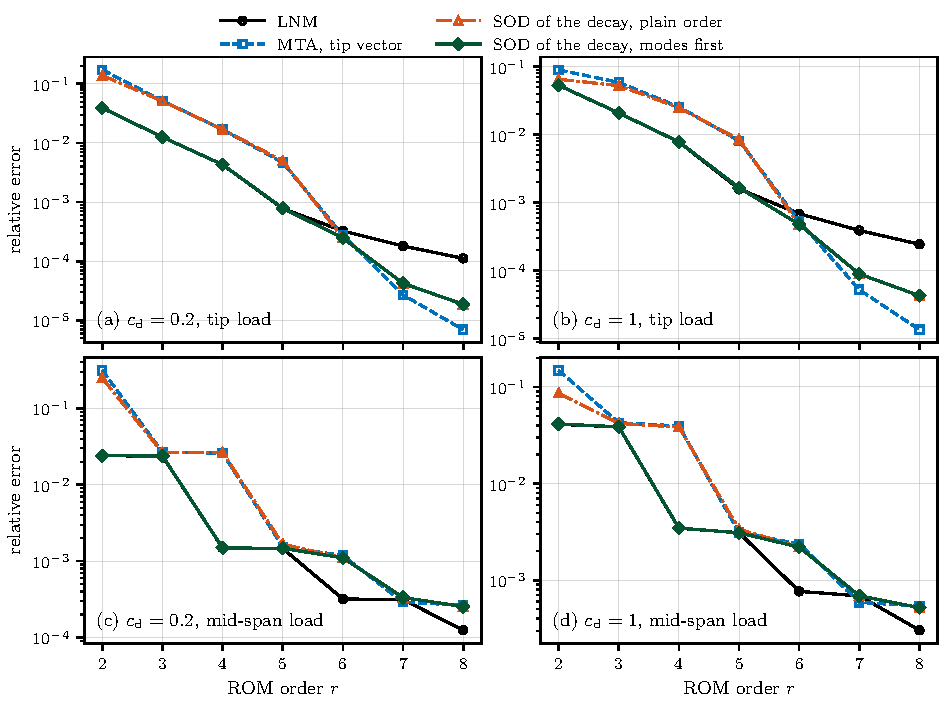
\includegraphics[width=\textwidth]{fig_v5_decay.pdf}
\caption{Cantilever with tip dashpot (S3): median ROM error over 20 random test loads against the ROM order. LNM; MTA with the tip static vector; and the SOD basis of the order-matched free decay, in plain SOD order and with the recognised modes first (Section~\ref{sec:order}). (a,b) Random load at the tip; (c,d) random load at mid-span. With the modes first, the SOD curve lies on the LNM curve at $r=2$--5.}
\label{fig:decay}
\end{figure}

\section{What the decay adds}\label{sec:decayadds}
If the hypothesis holds, the smooth modes of a decay are LNMs where no concentrated force acts, and S3 has one direction that is the tip-force response \eqref{eq:d}. Table~\ref{tab:angles} tests this on the order-8 decays, in the mass metric.

\paragraph{Rayleigh damping.} On S2 with light damping, smooth modes 1--5 lie $0.003^\circ$, $0.014^\circ$, $0.12^\circ$, $0.60^\circ$ and $2.0^\circ$ from LNMs 1--5, and the SOD frequencies are within 0.8\,\% of the natural frequencies. Modes 6--8, which the band-limited decay excites weakly, lie 4--$10^\circ$ away. No direction is non-modal.

\paragraph{Tip dashpot.} With $c_{\mathrm d}=0.2$ the decay has one more direction than modes in the band. Its SOD frequency, 69.4, lies between LNMs 3 and 4 (61.7 and 121). It is $16.7^\circ$ from the nearest LNM and $2.5^\circ$ from $\bm{d}(69.4)$ with $\bm{b}=\bm{e}_{\mathrm{tip}}$. With the dashpot force as $f$ in \eqref{eq:identity}, the force term carries 0.79 of that direction and the Rayleigh term 0.22, in mass norm. The other seven directions are LNMs 1--7, within $0.04$--$7^\circ$.
With $c_{\mathrm d}=1$ the extra direction sits at 110.3, $18.9^\circ$ from the nearest LNM and $4.0^\circ$ from $\bm{d}(110.3)$. Here the modal directions are themselves closer to the tip-force response than to the LNMs: the first lies $0.08^\circ$ from $\bm{d}$ and $0.64^\circ$ from LNM~1, the second $0.42^\circ$ and $4.4^\circ$. A strong dashpot bends every mode toward the response to its force.

\paragraph{Where the direction sits depends on the decay.} Each ROM order has its own decay, band-limited at $\omega_r$. For $c_{\mathrm d}=0.2$ the non-modal direction had SOD frequency 10.3, 22.8, 35.8, 44.6, 53.9, 63.3 and 70.2 for $r=2$ to 8. It was the second direction at $r=2$, the third at $r=3$--6 and the fourth at $r=7$ and 8. In every case it lay inside the first $r$.

\paragraph{Nonlinear springs.} On the decays of S4 and S5 the concentrated force is the cubic spring and the magnet force. The first four smooth modes of the S4 decay lie $3\times10^{-4}$, $0.008^\circ$, $0.04^\circ$ and $0.34^\circ$ from $\bm{d}$ at their SOD frequencies, and the force term carries 0.99--1.00 of each. The first three of the S5 decay lie $0.05^\circ$, $0.23^\circ$ and $0.60^\circ$ away (Section~\ref{sec:nonlin}).

\begin{table}[tbp]
\centering\small
\caption{Smooth modes of the order-8 band-limited free decays: SOD frequency $\sqrt{\mu_i}$, angle to the nearest LNM and angle to the tip-force response $\bm{d}(\sqrt{\mu_i})$, in degrees (mass metric). Bold: the non-modal direction. Script: \texttt{i4\_free\_decay\_identity.py}.}
\label{tab:angles}
\begin{tabular}{rrrrrrrrr}
\toprule
 & \multicolumn{2}{c}{S2, light Rayleigh} & \multicolumn{3}{c}{S3, $c_{\mathrm d}=0.2$} & \multicolumn{3}{c}{S3, $c_{\mathrm d}=1$}\\
\cmidrule(lr){2-3}\cmidrule(lr){4-6}\cmidrule(lr){7-9}
$i$ & $\sqrt{\mu_i}$ & LNM & $\sqrt{\mu_i}$ & LNM & $\bm{d}$ & $\sqrt{\mu_i}$ & LNM & $\bm{d}$\\ \midrule
1 & 3.51 & 0.003 & 3.42 & 0.04 & 0.04 & 2.53 & 0.64 & 0.08\\
2 & 22.0 & 0.014 & 22.0 & 0.28 & 0.11 & 21.2 & 4.4 & 0.42\\
3 & 61.6 & 0.12 & 61.4 & 0.56 & 0.41 & 60.7 & 2.3 & 0.88\\
4 & 121 & 0.60 & \textbf{69.4} & \textbf{16.7} & \textbf{2.5} & \textbf{110.3} & \textbf{18.9} & \textbf{4.0}\\
5 & 198 & 2.0 & 121 & 0.75 & 1.3 & 124 & 5.9 & 1.6\\
6 & 293 & 4.4 & 198 & 2.1 & 3.8 & 198 & 2.7 & 4.4\\
7 & 405 & 7.0 & 293 & 4.4 & 8.7 & 293 & 4.8 & 8.9\\
8 & 536 & 10.1 & 406 & 7.0 & 15.1 & 406 & 7.1 & 14.6\\
\bottomrule
\end{tabular}
\end{table}

\section{Why low orders fail, and how to recognise the modes}\label{sec:order}
\paragraph{One direction, ranked among the modes.} The non-modal direction always lay inside the first $r$ smooth modes, so a basis of order $r$ held $r-1$ modes and the force response. At low order the missing mode costs more than the force response buys: the plain-order basis lost a factor of 3.5--6.3 to the LNMs at $r=2$--5 on the tip load, and factors of 10.5 and 17.7 at $r=2$ and 4 on the mid-span load ($c_{\mathrm d}=0.2$). MTA-tip, which also spends one vector on the tip, lost the same factors (Figure~\ref{fig:decay}).

The remedy is to recognise the modes and place them first. We tested three routes on the S3 decays, at every order from 2 to 8, against LNM, CM and MTA-tip ROMs on the same 20 test loads.


\paragraph{Route 1, configuration SOD: spectral consistency.} A coordinate that is a single real mode has its mean-square frequency at its spectral peak. A mixture of modes does not. We read each coordinate's spectrum from its periodogram of the type-II discrete cosine transform (DCT-II), smoothed over $\pm2\,\%$ in frequency. A raw periodogram of a randomly forced coordinate has single-bin spikes. Its arg-max is then not the resonance, and its bin-level width misses the damping width $2\zeta\omega$. Coordinate $i$ is kept if its peak lies within $\max(5\,\%,\,w_i)$ of its SOD frequency $\sqrt{\mu_i}$. Here $w_i$ is the relative half-power width of that peak, capped at 15\,\%. The width makes the test damping-aware. The cap matters. A drifting or broadband coordinate peaks near zero frequency, with a width above 1, and would otherwise pass. The test assumes one frequency per coordinate. Two kept coordinates that share one peak cannot both be that mode. The one carrying more response energy, $\|\bphi_i\|^2\avg{q_i^2}$, is kept. Recognised modes are ordered by peak frequency.
Modes recognised inside the load band, $\omega\le\omega_{\mathrm c}$, are placed first, ordered by frequency; the rest follow in SOD order.
For $c_{\mathrm d}=0.2$ this removed the loss: the reordered basis gave 1.00, 1.00, 1.00 and 1.01 times the LNM error at $r=2$--5 and kept the gains at $r=6$--8. For $c_{\mathrm d}=1$ it failed at $r=2$--4. The first mode, with damping ratio 0.60, has no spectral peak at its SOD frequency and was not recognised; the reordered basis dropped it and the error was near 1 (\texttt{i5\_decay\_recognition.py}).


\paragraph{Route 2, state SOD: circularity.} Consider the two coordinates of a modal plane. Up to a real change of basis, they are the real and imaginary parts of one complex modal coordinate. SOD returns them uncorrelated and with unit variance, so in their own plane the cloud is round. Read as $z=q_a+\mathrm i\,q_b$, the pair rotates one way and the spectrum of $z$ is one-sided. Two unrelated coordinates, or coordinates of two different planes, give a nearly symmetric spectrum.
Pairs are therefore formed by matching, not by rank. Candidate pairs are paired greedily by one-sidedness and kept above 0.85; only one plane is kept per frequency. A loose frequency gate, four times the spectral tolerance, only limits the search. The plane frequency is the peak of the one-sided spectrum of $z$, and planes are ordered by it.
On the $c_{\mathrm d}=1$ decays circularity recognised all five planes in the band at every order, the first mode included (one-sidedness 0.86; the others 0.96--0.98). As a ROM basis, however, the state-SOD planes of a decay hold the modal planes and no force-response direction. The state ROM matched the LNMs at low order and then stalled: 2.3--8.4 times worse than the LNMs at $r=5$--8 for $c_{\mathrm d}=0.2$, and 5.9--24 times for $c_{\mathrm d}=1$ (\texttt{i6\_state\_recognition.py}; Section~\ref{sec:complex}).

\paragraph{Route 3: planes mark the modes of the configuration basis.} The two routes complement each other. Circularity recognises the modes; the configuration basis holds the force response. For each in-band plane found by circularity, we mark as modal the configuration smooth mode closest, in the mass metric, to the displacement part of the plane. The marked modes go first, ordered by plane frequency; the remaining directions follow in SOD order.
The marked mode lay within $2.1^\circ$ of its plane's displacement span wherever the plane's mode was inside the basis order. One plane beyond the basis order ($r=2$, $c_{\mathrm d}=1$) matched at $22.7^\circ$ and did not enter the ROM; a threshold of $5^\circ$ would have rejected it.
Table~\ref{tab:recog} and Figure~\ref{fig:decay} give the result. On the tip load the decay basis with modes first was within 4\,\% of the LNMs at $r=2$--5 and 1.3--6 times better at $r=6$--8, for both dashpots. On the mid-span load it equalled the LNMs at $r=2$--5. At $r=6$ and 8 it was 2.9--3.5 and 1.7--2.0 times worse than the LNMs, as MTA-tip was: the tip-force response had displaced a mode that the mid-span load excites (\texttt{i7\_hybrid\_recognition.py}).

\begin{table}[tbp]
\centering\small
\caption{S3: median over 20 realizations of the ROM error divided by the LNM error, random tip load. Plain: SOD order. Modes first: Route 3. Scripts: \texttt{i5\_decay\_recognition.py}, \texttt{i7\_hybrid\_recognition.py}.}
\label{tab:recog}
\begin{tabular}{llrrrrrrr}
\toprule
dashpot & order of the decay basis & $r=2$ & 3 & 4 & 5 & 6 & 7 & 8\\ \midrule
$c_{\mathrm d}=0.2$ & plain & 3.48 & 4.07 & 3.98 & 6.33 & 0.76 & 0.23 & 0.17\\
 & modes first & 1.00 & 1.00 & 1.00 & 1.01 & 0.76 & 0.23 & 0.17\\
$c_{\mathrm d}=1$ & plain & 1.23 & 2.50 & 3.14 & 5.35 & 0.69 & 0.23 & 0.17\\
 & modes first & 1.00 & 1.00 & 1.00 & 1.04 & 0.69 & 0.23 & 0.17\\
\bottomrule
\end{tabular}
\end{table}

\section{Nonlinear cantilevers}\label{sec:nonlin}
A local nonlinear spring is a concentrated internal force, like the dashpot. Does the same explanation account for what a decay-trained basis gains there? S4 tests backbone accuracy and S5 forced bifurcations.


\subsection{A nonlinear backbone}\label{sec:nlbb}
Nonlinear ROMs proper reduce onto invariant manifolds: nonlinear normal modes \citep{Shaw1993,Touze2004} and spectral submanifolds \citep{Haller2016,Cenedese2022}. Model-based alternatives augment the modes with static or derivative vectors, or with a quadratic manifold built from them \citep{Idelsohn1985,Jain2017}; \citet{Mignolet2013} review non-intrusive ROMs of geometrically nonlinear structures, including the choice of basis; \citet{Touze2021} review invariant-manifold methods and the quadratic manifold. We do not compete with them. We test linear Galerkin bases only, where SOD is an alternative to LNM, MTA and POD. We compare linear Galerkin bases only.
S4 is the COST F3 cantilever of Section~\ref{sec:bench} (Figure~\ref{fig:systems}d).

\paragraph{Reference backbone.} We computed the NNM1 backbone \citep{Kerschen2009} of the full model by odd harmonic balance \citep{Detroux2015}. It used eight harmonics and pseudo-arclength continuation.
We integrated the full model over one period from the balanced initial state, at four energies. It returned to that state within $1.5\times10^{-10}$ or better.
The backbone rises from 23.66\,Hz to 42.1\,Hz at total energy $H=3\times10^{-2}$\,J.
A 5:1 internal resonance with mode 2 (148.3\,Hz) forms a tongue at 29.9--30.4\,Hz (Figure~\ref{fig:nl}a). The main backbone is interrupted between $H=3.6\times10^{-3}$ and $4.0\times10^{-3}$\,J, where the tongue branches off. The tongue itself stays near 30\,Hz up to the highest energy computed.
There the fifth harmonic exceeds the fundamental. We compare backbones outside the tongue only.
Plucked responses from static deflections are not on the backbone. Their zero-crossing frequencies lay up to 3\,\% below it at the same energy. The plucked state also excites higher modes.

\paragraph{Bases.} LNM; MTA with the static tip-load vector; and SOD and POD of one damped decay ($\zeta=0.01$, Rayleigh on modes 1--2). Two decays were used. The band-limited decay follows the convention of Section~\ref{sec:bench}. It is an equal-energy sum of LNMs 1--4, the band of interest for $r\le4$. The static-release decay starts from the deflection under a 30\,N tip load. The results below are for static release; the band-limited decay follows them. It lasts 1.5\,s and sweeps the energy down the backbone.
Each ROM backbone was computed by the same harmonic balance on the reduced equations.

\paragraph{Results.} Median backbone frequency errors over 24 energies outside the tongue, from $6\times10^{-4}$ to $2.5\times10^{-2}$\,J (Figure~\ref{fig:nl}b):
\begin{itemize}
\item $r=1$: LNM $1.1\times10^{-2}$, SOD and POD $2.2\times10^{-3}$;
\item $r=2$: LNM $1.5\times10^{-3}$, MTA $8\times10^{-5}$, SOD $1.4\times10^{-4}$, POD $2.1\times10^{-4}$;
\item $r=3$: LNM $4.7\times10^{-4}$, MTA $1.4\times10^{-6}$, SOD $2.0\times10^{-6}$, POD $1.2\times10^{-5}$;
\item $r=4$: LNM $2.0\times10^{-4}$, MTA $1.4\times10^{-6}$, SOD $5\times10^{-7}$, POD $4\times10^{-7}$.
\end{itemize}
At $r=3$ and 4, decay-trained bases improved the backbone by two to three decades over the LNMs. At $r=2$ the gain was about one decade. The model-based static tip-load vector did as well or better at $r=2$ and 3. At $r=4$ the order of SOD and MTA depends on the energy range: over the longer backbone of Section~\ref{sec:s-s4} the medians were $4.8\times10^{-7}$ for MTA and $6.0\times10^{-7}$ for SOD.
Both contain the deformation that the localized cubic force imposes on the beam: MTA as $\bK^{-1}\bm{e}_{\mathrm{tip}}$, SOD in its smooth modes. By \eqref{eq:identity} with the cubic force as $f$, each is the tip-force response $\bm{d}$ at its own SOD frequency: the first four lie $3\times10^{-4}$, $0.008$, $0.04$ and $0.34$ degrees from $\bm{d}$ at 196.0, 839, 1249 and 2859\,rad/s, and the force term carries 0.99--1.00 of each (\texttt{i1\_forced\_identity.py}). The first lies $2.6^\circ$ from the static vector and $1.1^\circ$ from LNM~1.
SOD led POD at $r=2$ and 3; at $r=4$ POD was 1.4 times better.

\paragraph{Held-out time-domain tests.} Conservative responses started from static deflections not used in training. The loads were 3, 10 and 20\,N at the tip and 20 and 60\,N at mid-span.
At $r=4$, MTA, SOD and POD gave displacement errors of $1.5$--$5.5\times10^{-3}$ over 0.1\,s. The LNMs gave $4.5\times10^{-4}$ to $1.1\times10^{-2}$, better at low energy and worse at high energy. Zero-crossing frequency errors were at most $1.1\times10^{-4}$ for SOD and MTA, and up to $9.1\times10^{-4}$ for the LNMs.
At $r=2$, displacement errors were $0.58$--$3.8\times10^{-2}$ for POD, $0.8$--$4.8\times10^{-2}$ for SOD, $0.42$--$8.4\times10^{-2}$ for the LNMs and $4$--$13\times10^{-2}$ for MTA.
The plucked states excite modes that a backbone-dominated record does not contain. At $r=4$ displacement accuracy in these tests was therefore limited by the truncated modes: MTA, SOD and POD gave errors within the same range.
The four-mode SOD ROM matched the backbone to about $10^{-6}$ up to 0.048\,J, about three times the $1.48\times10^{-2}$\,J of its training state; there an internal-resonance tongue of the ROM itself begins (Figure~\ref{fig:track}). Section~\ref{sec:s-s4} gives the band-limited training decay, the backbone read from the record alone, the out-of-plane bend of the NNM and the integration cost.

\paragraph{The bent correction as a basis vector.} With $(\bK-\omega^2\bM)^{-1}\bm{e}_{\mathrm{tip}}$ at $\omega=196.0$\,rad/s in place of the static vector, the one-mode ROM equalled the one-mode SOD ROM ($2.2\times10^{-3}$). At $r=2$ it was the most accurate basis: backbone error $4.7\times10^{-5}$, against $8.0\times10^{-5}$ for MTA and $1.4\times10^{-4}$ for SOD. At $r=3$ and 4 it equalled MTA, $1.4\times10^{-6}$. The model-built basis of $\bm{d}$ at the first $r$ SOD frequencies gave $2.2\times10^{-3}$, $1.6\times10^{-4}$, $4.9\times10^{-6}$ and $1.4\times10^{-6}$ for $r=1$--4, against $2.2\times10^{-3}$, $1.4\times10^{-4}$, $2.0\times10^{-6}$ and $5.2\times10^{-7}$ for SOD: equal at $r=1$, within 1.2 at $r=2$, and 2.5--2.7 times worse at $r=3$ and 4 over this energy range (Section~\ref{sec:s-s4}).

\begin{figure}[tbp]
\centering
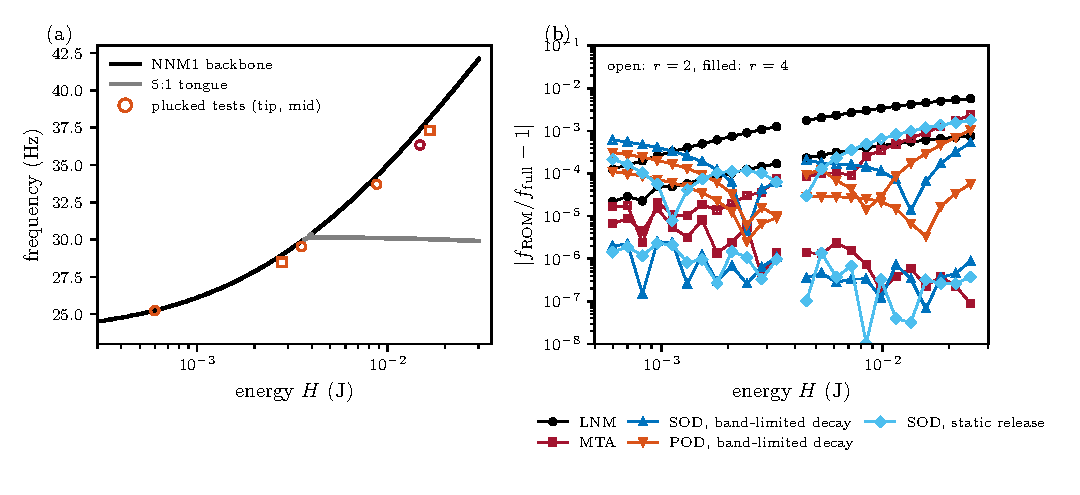
\includegraphics[width=\textwidth]{fig_c_nl.pdf}
\caption{COST F3 cantilever with cubic tip spring. (a) Frequency--energy plot of NNM1 from harmonic balance: main backbone, 5:1 tongue, and zero-crossing frequencies of the plucked tests. Circles: tip loads; squares: mid-span loads; dark: the 30\,N training state. (b) Backbone frequency error of the ROMs against energy, outside the tongue; open: $r=2$, filled: $r=4$. SOD and POD from the band-limited decay (LNMs 1--4, equal energy), and SOD from the static release.}
\label{fig:nl}
\end{figure}

\subsection{Bifurcation diagrams of a two-well beam}\label{sec:moon}
A backbone tests free motion on one NNM. Forced motion between two potential wells is harder. It has coexisting attractors, period doubling and chaos. S5 is a cantilever of this kind, after the magneto-elastic beam of \citet{Moon1979}.

\paragraph{Model.} Ten Hermite elements, $EI=m'=L=1$ as for S2, $n=20$. A tip force $f=-k_1x+k_3x^3$, with $x$ the tip deflection, $k_1=6$ and $k_3=300$, stands in for the magnets. Since $k_1$ exceeds the tip stiffness $3EI/L^3$, the straight state is unstable. Two buckled equilibria have tip deflection $\pm x^*=\pm0.1$. Linearized there, the first three frequencies are $\omega_{\mathrm w}=4.90$, 22.3 and 61.8; the clamped beam has 3.52, 22.0 and 61.7. Rayleigh damping gives $\zeta=0.02$ at the first two well modes. The base acceleration is $A\cos\varOmega t$. All models were integrated by average-acceleration Newmark \citep{Newmark1959} with Newton iterations, at 100 steps per forcing period.

\paragraph{Training and bases.} One cross-well free decay trained the data bases. It started at $+x^*$ with the velocity of a unit step in base velocity. Over 60 time units the tip swept $\pm2.5x^*$ and crossed zero 18 times, the last at $t=14.1$. It then settled in a well. Velocities came from the model.
\begin{itemize}
\item POD and SOD used second moments about zero, so the buckled equilibria stay in the span. The data rank was 11.
\item The first POD direction held 98.7\,\% of the variance. The SOD frequencies were 2.49, 10.4, 23.8 and 60.8. The second SOD direction is not modal: its MAC with the second well LNM was 0.05.
\item MTA used $r-1$ clamped LNMs plus $\bK^{-1}\bm{e}_{\mathrm{tip}}$, the static vector of the nonlinear force. Two LNM bases were also tested: clamped, and linearized in a well.
\end{itemize}
The first SOD direction lies $0.7^\circ$ from $\bK^{-1}\bm{e}_{\mathrm{tip}}$ in the mass metric.

\paragraph{Diagrams.} The forcing parameter was swept up and down. The state was carried from one value to the next. After a transient, the tip displacement was sampled once per period at phase $\varOmega t=0 \bmod 2\uppi$. A response is called periodic of period $k$ if it has $k$ distinct samples to $10^{-3}x^*$. It is cross-well if its orbit changes sign. ROM and full-model sample sets were compared by their Wasserstein distance $W_1$, divided by $x^*$. In-well orbits were also compared by their extremes. A ROM may settle on the mirror orbit, $-x(t+\uppi/\varOmega)$, in the other well. That is a choice between coexisting attractors, not a model error, so the mirror orbit is compared instead.

\paragraph{Amplitude sweep.} At $\varOmega=0.85\,\omega_{\mathrm w}$, $A$ ran from 0.01 to 0.30 in steps of $10^{-3}$, with 150 transient and 64 sampled periods (Figure~\ref{fig:mbamp} of the supplement). The cascade was resolved in steps of $10^{-4}$ with 300 transient periods (Figure~\ref{fig:mbcasc}). On the up sweep the full model showed:
\begin{itemize}
\item a small in-well orbit, which jumped to a resonant in-well orbit at $A=0.075$;
\item period doubling at $A=0.1286$ (period 2), 0.1396 (period 4) and 0.1410 (period 8);
\item escape to cross-well chaos at 0.1412, a period-5 window at 0.173--0.181, and cross-well period-1 motion above 0.238.
\end{itemize}
Period 16 lay within one step of $10^{-4}$. On the down sweep, cross-well period-1 motion persisted to $A=0.093$.

\paragraph{One mode.} One-mode ROMs reproduced the sequence but shifted it in amplitude. The onset of period 2 moved by $-1.5\,\%$ (SOD), $-1.3\,\%$ (POD) and $-5.6\,\%$ (MTA). It moved by $+4.4\,\%$ (clamped LNM) and $+18\,\%$ (LNM in the well). The escape moved by about as much. The shift follows the one-mode model itself. With $\bphi$ scaled to unit tip displacement, it reads $\bar m\ddot q+\bar c\dot q+(\bar k-k_1)q+k_3q^3=-\varGamma\bar m\,a_{\mathrm g}$. Here $\bar m$, $\bar c$ and $\bar k$ are the modal mass, damping and stiffness, $\varGamma$ is the participation factor and $a_{\mathrm g}$ the base acceleration. Its equilibrium is $q^*=\sqrt{(k_1-\bar k)/k_3}$ and its well frequency $\sqrt{2(k_1-\bar k)/\bar m}$ (Table~\ref{tab:moon}). The static vector gives the exact equilibrium but a light modal mass, so its well frequency is 3.0\,\% high. The LNM in the well is 9.3\,\% low. SOD balances the two errors. A high well frequency moved the cascade to lower amplitude, and a low one to higher amplitude.


\paragraph{Which vector is the first SOD direction?} The magnets act as a rank-one stiffness at the tip. The deflection under a harmonic tip force at frequency $\omega$, $\bm{d}(\omega)=(\bK-\omega^2\bM)^{-1}\bm{e}_{\mathrm{tip}}$, therefore runs from the static vector at $\omega=0$ to the in-well LNM at $\omega=\omega_{\mathrm w}$: the in-well mode satisfies $(\bK-\omega_{\mathrm w}^2\bM)\bphi=-\kappa\phi_{\mathrm{tip}}\bm{e}_{\mathrm{tip}}$, with $\kappa$ the linearized magnet stiffness. The first SOD direction lies on this curve. It is $0.69^\circ$ from $\bm{d}(0)$, $2.2^\circ$ from $\bm{d}(\omega_{\mathrm w})$, and $0.003^\circ$ from $\bm{d}(2.417)$; at the first SOD frequency, 2.49, the angle is $0.05^\circ$, as \eqref{eq:identity} predicts with the magnet force as $f$; the record-end term carries 0.04 of the direction, because this decay starts with a velocity (\texttt{mb10\_dynamic\_correction.py}, \texttt{i1\_forced\_identity.py}). With $\bm{d}(2.417)$ as its one vector, a one-mode ROM reproduced SOD: equilibrium $-0.32\,\%$ and well frequency $+1.26\,\%$, against $-0.32\,\%$ and $+1.25\,\%$. On the amplitude sweep its in-well extreme error was $1.38\times10^{-2}$, against $1.37\times10^{-2}$ for SOD and $2.56\times10^{-2}$ for MTA, and its cascade landmarks matched those of SOD at the sweep step of $10^{-3}$. The one-mode advantage of SOD over MTA is therefore the static correction bent by inertia at the frequency of the training record.

\paragraph{More modes.} At $r=2$ SOD, POD and MTA placed the period-2, period-4 and escape amplitudes within one step of $10^{-4}$; the two LNM bases still erred by 0.6--3\,\%. Which of SOD and MTA is closer at $r=2$ depends on the measure: SOD erred less on the in-well orbit extremes ($1.5\times10^{-4}$ against $3.3\times10^{-4}$), MTA on the in-well Wasserstein distance ($2.0\times10^{-5}$ against $7.9\times10^{-5}$; Table~\ref{tab:s-moon}). Replacing the static vector of MTA by $\bm{d}(2.417)$ did not move it toward SOD on the extremes ($3.1\times10^{-4}$). On the amplitude sweep MTA was the most accurate basis from $r=3$ and SOD second (Table~\ref{tab:moon}). Classification agreed with the full model at 98.5--99.5\,\% of the 582 points for SOD, MTA and POD at $r\ge2$. The remaining points lie at the edges of the chaotic windows.

\paragraph{Frequency sweep.} At $A=0.3$, $\varOmega$ ran from 0.2 to 1.4 $\omega_{\mathrm w}$ (Section~\ref{sec:s-s5}). At $r\ge2$ every ROM placed the jumps into and out of cross-well motion within $0.04\,\omega_{\mathrm w}$, SOD and MTA were within a factor of 1.2 at $r=3$ ($1.8\times10^{-6}$ and $2.1\times10^{-6}$), and MTA led by 1.9 at $r=4$ (Table~\ref{tab:moon}).

\begin{table}[tbp]
\centering\small
\caption{Two-well beam (S5). One-mode ROMs: relative errors of the equilibrium $q^*$ and the well frequency. Then the median error of the response against $r$. Amplitude sweep: in-well orbit extremes, divided by $x^*$. Frequency sweep: $W_1/x^*$ on the periodic points.}
\label{tab:moon}
\setlength{\tabcolsep}{3pt}
\resizebox{\textwidth}{!}{\begin{tabular}{lrrcccccccc}
\toprule
 & \multicolumn{2}{c}{one mode} & \multicolumn{4}{c}{amplitude sweep, $r=1$--4} & \multicolumn{4}{c}{frequency sweep, $r=1$--4}\\
\cmidrule(lr){2-3}\cmidrule(lr){4-7}\cmidrule(lr){8-11}
basis & $q^*$ & $\omega_{\mathrm w}$ & 1 & 2 & 3 & 4 & 1 & 2 & 3 & 4\\ \midrule
SOD & $-0.3\,\%$ & $+1.3\,\%$ & $1.4\times10^{-2}$ & $1.5\times10^{-4}$ & $8.5\times10^{-7}$ & $3.3\times10^{-8}$ & $2.0\times10^{-2}$ & $1.4\times10^{-3}$ & $1.8\times10^{-6}$ & $1.8\times10^{-7}$\\
POD & $-0.3\,\%$ & $+1.2\,\%$ & $1.4\times10^{-2}$ & $1.5\times10^{-4}$ & $1.1\times10^{-5}$ & $3.8\times10^{-7}$ & $2.2\times10^{-2}$ & $1.0\times10^{-3}$ & $3.5\times10^{-5}$ & $2.8\times10^{-6}$\\
MTA & $0$ & $+3.0\,\%$ & $2.6\times10^{-2}$ & $3.3\times10^{-4}$ & $2.4\times10^{-7}$ & $4.8\times10^{-9}$ & $1.8\times10^{-2}$ & $2.2\times10^{-3}$ & $2.1\times10^{-6}$ & $9.6\times10^{-8}$\\
LNM, clamped & $-1.5\,\%$ & $-1.5\,\%$ & $2.0\times10^{-2}$ & $3.1\times10^{-3}$ & $9.6\times10^{-4}$ & $4.1\times10^{-4}$ & $2.2\times10^{-2}$ & $2.2\times10^{-3}$ & $7.5\times10^{-4}$ & $3.0\times10^{-4}$\\
LNM, in well & $-6.5\,\%$ & $-9.3\,\%$ & $1.2\times10^{-1}$ & $1.5\times10^{-2}$ & $4.5\times10^{-3}$ & $1.9\times10^{-3}$ & $3.1\times10^{-2}$ & $5.5\times10^{-3}$ & $1.4\times10^{-3}$ & $6.1\times10^{-4}$\\
\bottomrule
\end{tabular}}
\end{table}

\begin{figure}[tbp]
\centering
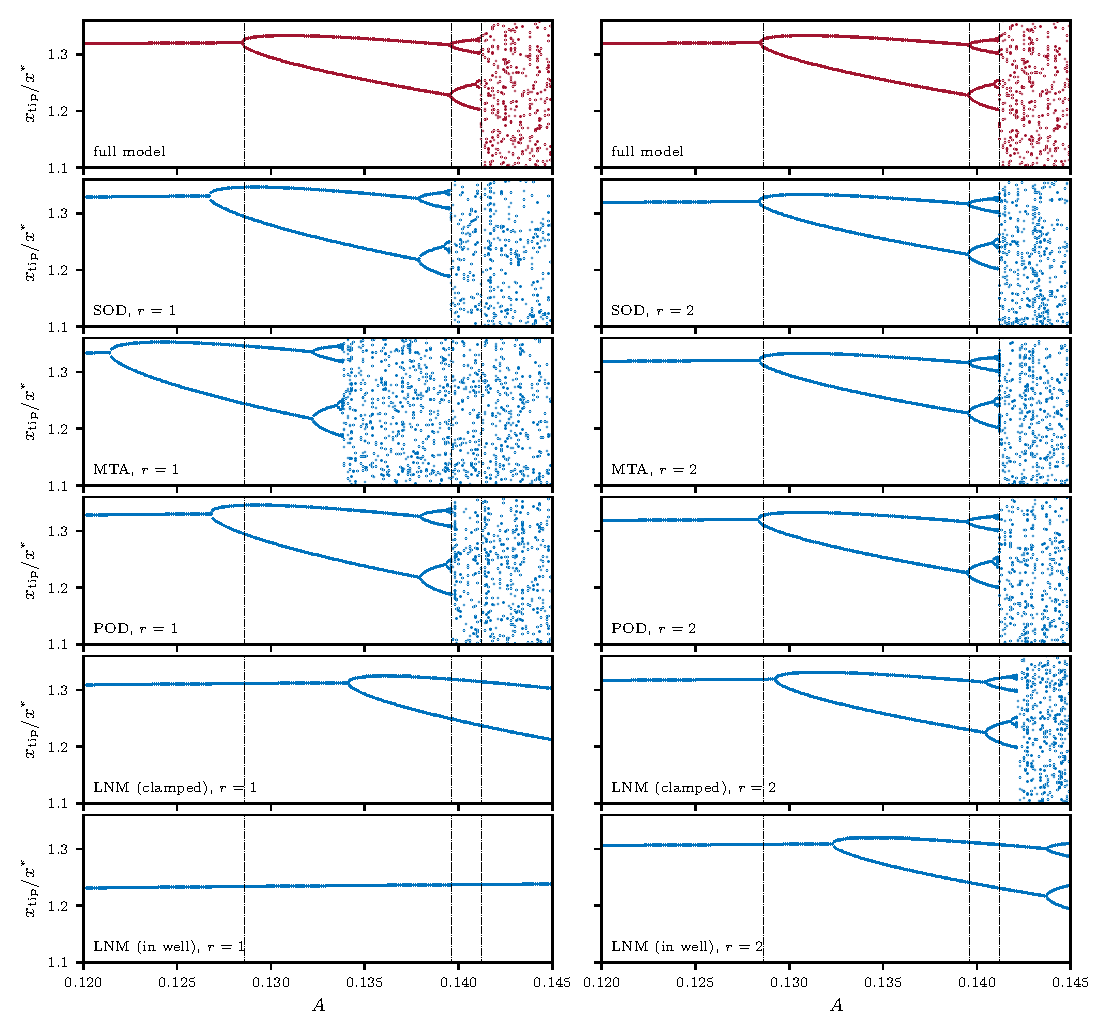
\includegraphics[width=\textwidth]{fig_mb_cascade.pdf}
\caption{The period-doubling cascade of Figure~\ref{fig:mbamp}, up sweep in steps of $10^{-4}$. ROMs on the mirror orbit are shown through it. Dotted: full-model onsets of period 2 and period 4, and the escape to cross-well motion. Left $r=1$, right $r=2$. The cascade of the in-well LNM ROM at $r=1$ lies above $A=0.15$.}
\label{fig:mbcasc}
\end{figure}

\paragraph{What the two-well beam adds.} It shows where model-based correction accounts for the data advantage. One cross-well decay gave SOD the correction at the nonlinear force without its location. At one mode that correction is bent by inertia at the record's frequency, and it beats the static vector; the same bent vector, built from the model, does as well. At $r=2$ SOD and MTA trade places by measure. On the amplitude sweep the model-based MTA basis was the most accurate from $r=3$, with SOD within a factor of 7; on the frequency sweep the two were within a factor of 2. POD fell behind both.


\section{Contrasts: forced training records and heavy proportional damping}\label{sec:contrast}
\paragraph{A forced record adds the response to its load.} An external load is a concentrated force too, and \eqref{eq:identity} applies with the load as $f$. On S2 with light damping, SOD of a random tip-load record had one non-modal direction near 50\,rad/s, between LNMs 2 and 3. At $r=8$ its subspace contained the static tip vector to a residual of $1.8\times10^{-7}$, against $3.3\times10^{-5}$ for the LNMs and $3.6\times10^{-5}$ for the decay basis. Its ROM was 27 times more accurate than the LNM ROM at $r=8$ on a new tip load, 4.8 times less accurate at $r=3$, and no better under a mid-span load (Sections~\ref{sec:acc}--\ref{sec:displace}). A model-built basis of the load responses $\bm{d}$ at the record's SOD frequencies reproduced the SOD ROM errors within factors of 0.82--1.21 at every order from 1 to 8 (20 realizations; Section~\ref{sec:s-forced}). The decay basis lacks this direction because a free decay has no load: it learns the structure's own concentrated forces, not the loads the ROM will meet.

\paragraph{Heavy proportional damping biases the decay modes.} With heavy Rayleigh damping ($\zeta=0.20$ at modes 1 and 4) the smooth modes of the S2 decay lay $0.16^\circ$, $0.69^\circ$, $4.8^\circ$ and $15^\circ$ from LNMs 1--4, and 28--$48^\circ$ for modes 5--8. The decay ROM was up to 1.75 times less accurate than the LNM ROM (at $r=8$; 1.27 at $r=5$) on the tip load. The damping term of \eqref{eq:identity} is then not small, and for distributed damping it is not a response to a force at one point.


\section{Discussion}\label{sec:disc}
The evidence supports the hypothesis on every decay tested. With Rayleigh damping at $\zeta=0.02$ the decay basis is the LNM basis: smooth modes within $2^\circ$ of LNMs 1--5 and ROM errors within 12\,\%. With a tip dashpot it has exactly one more direction, $17$--$19^\circ$ from any LNM and $2.5$--$4^\circ$ from the response to a tip force at its own SOD frequency. On the two nonlinear decays the smooth modes lie within $0.34^\circ$ (S4, four modes) and $0.60^\circ$ (S5, three modes) of that response. The identity \eqref{eq:identity} gives the reason and names the corrections: the remaining damping and the record ends.

The ROM consequences agree. In plain order the dashpot-decay basis tracked MTA-tip within a factor of 1.2 at $r=2$--6, and MTA-tip was 2.7 times better at $r=8$. What the decay supplies is therefore what static correction supplies, with one difference in the input: MTA must be told where the force acts, and the decay finds it. The difference in the output is that the decay's direction is the force response at a frequency the record sets, not at zero frequency. On S5 that frequency accounted for the one-mode advantage of SOD over MTA. On S4 the model-built responses at the SOD frequencies matched SOD at $r=1$ and 2 and were 2.5--2.7 times worse at $r=3$ and 4 over the reported energy range; over a longer backbone the order of SOD and MTA at $r=4$ reversed. We draw no conclusion from differences of that size on S4.

The low-order loss is the cost of ranking. The force-response direction enters among the modes, and the basis of order $r$ holds $r-1$ of them. Recognition by spectral consistency removed the loss for the light dashpot and failed for a mode with damping ratio 0.60. Circularity recognised that mode, but the state-SOD basis has no force-response direction. Marking the configuration modes through the recognised planes removed the loss in both cases, at every order from 2 to 5, and kept the gain from 6. The rule needs accelerations for the state derivative; in model reduction they come from the model.

The gain is specific to where the force acts. Under a mid-span load the decay basis of S3 was 1.7--3.5 times worse than the LNMs at $r=6$ and 8, as MTA-tip was. A free decay teaches the basis the structure's internal concentrated forces. It does not teach it the external loads; a forced record does, at its own load location (Section~\ref{sec:contrast}).

What the evidence does not show is the same mechanism on measured records. Every record here is full-field with model velocities. On a structure the force-response direction must be observable at the sensors, and velocities must be estimated.

\paragraph{Limitations.} All data are simulated and full-field, with model velocities and accelerations; sensor coverage and estimated kinematics were not tested. Each benchmark has one concentrated internal force, at the tip; several forces, or a distributed nonlinearity whose force pattern changes with amplitude, were not tested. The dashpot tests use one beam, two dashpot coefficients, one decay per order and 20 test loads; the nonlinear tests use one training decay each. Heavy proportional damping biased the decay modes by up to $48^\circ$, and the decay ROM was then up to 1.75 times worse than the LNM ROM. The marking rule was applied without an angle threshold. We tested linear Galerkin bases only, with no manifold-based ROM \citep{Haller2016,Jain2017} for comparison.

\section{Conclusions}\label{sec:concl}
A free decay teaches an SOD basis the modes and the structure's concentrated internal forces. With light Rayleigh damping the decay basis was the LNM basis. With a tip dashpot, a cubic tip spring or a two-well tip force it held, in addition, the response to a force at that point at the direction's own SOD frequency; a covariance identity with the force term kept gives this result and its damping and record-end corrections. The low-frequency limit of that response is the static vector of MTA, and the decay-trained ROMs tracked MTA-tip, without the force location being supplied.
SOD ranks the force-response direction among the modes, and a truncated basis then loses a mode: 3.5--6.3 times the LNM error at two to five modes on the dashpot beam. With the modal directions marked by the circular planes of state-space SOD and placed first, the decay basis equalled the LNMs at two to five modes and was up to 6 times better from six, for dashpots giving first-mode damping ratios of 0.13 and 0.60. The gain holds for loads the tip-force response serves; under a mid-span load the basis was 1.7--3.5 times worse than the LNMs at six and eight modes.


\appendix
\section{Proofs}\label{app:proofs}

\paragraph{Configuration SOD.} Let $\bx=\bPhi\bm{\eta}$, with $\bPhi$ the mass-normalized LNMs, and assume full-rank data. Then $\bSig_x=\bPhi\bm{G}_x\bPhi^{\mathsf T}$ and $\bSig_v=\bPhi\bm{G}_v\bPhi^{\mathsf T}$. Put $\bpsi=\bPhi^{-\mathsf T}\bm{\chi}$. The pencil $\bSig_v\bpsi=\mu\bSig_x\bpsi$ becomes
\begin{equation}
\bm{G}_v\bm{\chi}=\mu\,\bm{G}_x\bm{\chi},\qquad \bphi=\bSig_x\bpsi=\bPhi\bm{G}_x\bm{\chi} .
\label{eq:app_modal}
\end{equation}
\begin{itemize}
\item \emph{Sufficiency.} If $\bm{G}_x$ and $\bm{G}_v$ are diagonal, $\bm{\chi}_i\propto\bm{e}_i$. Then $\bphi_i\propto\bPhi\bm{e}_i$, the $i$th LNM, and $\mu_i=(\bm{G}_v)_{ii}/(\bm{G}_x)_{ii}$.
\item \emph{Necessity.} Let every $\bphi_i$ be an LNM and the $\mu_i$ distinct. Then $\bm{G}_x\bm{\chi}_i\propto\bm{e}_i$, so $\bm{\chi}_i\propto\bm{G}_x^{-1}\bm{e}_i$. The $\bm{\chi}_i$ are $\bm{G}_x$-orthogonal, hence $\bm{e}_i^{\mathsf T}\bm{G}_x^{-1}\bm{e}_j=0$ for $i\ne j$. So $\bm{G}_x^{-1}$, and with it $\bm{G}_x$, is diagonal. Then $\bm{\chi}_i\propto\bm{e}_i$, and \eqref{eq:app_modal} makes $\bm{G}_v$ diagonal.
\item \emph{Frequencies.} With both diagonal, $\mu_i=\omega_i^2$ if and only if $(\bm{G}_v)_{ii}=\omega_i^2(\bm{G}_x)_{ii}$. Write $(\bm{G}_v)_{ii}=\omega_i^2(1+\delta_i)(\bm{G}_x)_{ii}$. Then $\sqrt{\mu_i}=\omega_i(1+\delta_i)^{1/2}=\omega_i(1+\delta_i/2+O(\delta_i^2))$, and the mode is unchanged.
\item \emph{Correlation.} Let the off-diagonal entries of $\bm{G}_x$ and $\bm{G}_v$ be of order $\epsilon$. Standard perturbation of \eqref{eq:app_modal} gives $\bm{\chi}_i=\bm{e}_i+\sum_{j\ne i}c_{ij}\bm{e}_j+O(\epsilon^2)$. Here $c_{ij}=[(\bm{G}_v)_{ji}-\mu_i(\bm{G}_x)_{ji}]/[(\mu_i-\mu_j)(\bm{G}_x)_{jj}]$. The mode rotates at first order; $\mu_i$ changes at second order.
\end{itemize}

\paragraph{Defect of a damped decay.} Take $\ddot\eta+2\zeta\omega\dot\eta+\omega^2\eta=0$ with $\eta(0)=\hat\eta\cos\varphi$, $\dot\eta(0)=-\omega\hat\eta\sin\varphi$, and $0<\zeta<1$. Let $I_x=\int_0^\infty\eta^2\,\mathrm{d}t$ and $I_v=\int_0^\infty\dot\eta^2\,\mathrm{d}t$. Multiply the equation by $\dot\eta$ and integrate; then multiply by $\eta$ and integrate. The boundary terms give
\begin{equation}
I_v=\frac{\omega\hat\eta^2}{4\zeta},\qquad
\omega^2 I_x=I_v\left(1+4\zeta^2\cos^2\varphi-2\zeta\sin2\varphi\right).
\end{equation}
Thus $\mu=I_v/I_x=\omega^2/(1+4\zeta^2\cos^2\varphi-2\zeta\sin2\varphi)$. Released from rest ($\varphi=0$), $\mu=\omega^2/(1+4\zeta^2)$: the defect is $-4\zeta^2/(1+4\zeta^2)$, second order in $\zeta$. With an initial velocity the first-order term $-2\zeta\sin2\varphi$ appears; it averages to zero over $\varphi$. The infinite horizon stands for a record that has decayed.

\paragraph{Proposition~\ref{prop:ssod}.} Consider a free response, $\dot{\bm{y}}=\bm{A}\bm{y}$. In real modal coordinates $\bm{y}=\bm{P}\bm{\xi}$, $\dot{\bm{\xi}}=\bm{L}\bm{\xi}$ with $\bm{L}=\operatorname{blockdiag}(\bm{L}_i)$. Assume $\bm{P}$ invertible and $\avg{\bm{\xi}\bm{\xi}^{\mathsf T}}=\bm{G}=\operatorname{blockdiag}(\bm{G}_i)$ with each $\bm{G}_i\succ0$. Then $\avg{\bm{y}\bm{y}^{\mathsf T}}=\bm{P}\bm{G}\bm{P}^{\mathsf T}$ and $\avg{\dot{\bm{y}}\dot{\bm{y}}^{\mathsf T}}=\bm{P}\bm{L}\bm{G}\bm{L}^{\mathsf T}\bm{P}^{\mathsf T}$. With $\bpsi=\bm{P}^{-\mathsf T}\bm{\chi}$, the pencil \eqref{eq:ssod} becomes
\begin{equation}
\bm{L}\bm{G}\bm{L}^{\mathsf T}\bm{\chi}=\mu\,\bm{G}\bm{\chi} .
\end{equation}
Both sides are block diagonal, so the pencil splits into $2\times2$ pencils $\bm{L}_i\bm{G}_i\bm{L}_i^{\mathsf T}\bm{\chi}=\mu\bm{G}_i\bm{\chi}$.
\begin{itemize}
\item \emph{Pair product.} $\mu_{i,a}\mu_{i,b}=\det(\bm{L}_i\bm{G}_i\bm{L}_i^{\mathsf T})/\det\bm{G}_i=(\det\bm{L}_i)^2=|s_i|^4$.
\item \emph{Span.} An eigenvector $\bm{\chi}$ of plane $i$ is zero outside that block. Its smooth mode $\bphi=\bm{P}\bm{G}\bm{\chi}$ lies in the span of $\bm{P}_i=(\operatorname{Re}\,\bm{v}_i,\operatorname{Im}\,\bm{v}_i)$.
\item \emph{Equal values.} Write $\bm{L}_i=\sigma_i\bm{I}+\omega_i\bm{J}$ with $\bm{J}=\big[\begin{smallmatrix}0&1\\-1&0\end{smallmatrix}\big]$, and $\bm{S}=\bm{G}_i^{1/2}$. The two values are equal if and only if $\bm{D}\bm{D}^{\mathsf T}=\mu\bm{I}$, where $\bm{D}=\bm{S}^{-1}\bm{L}_i\bm{S}=\sigma_i\bm{I}+\omega_i\bm{N}$ and $\bm{N}=\bm{S}^{-1}\bm{J}\bm{S}$. If $\bm{G}_i\propto\bm{I}$, then $\bm{N}=\bm{J}$ and $\bm{D}\bm{D}^{\mathsf T}=|s_i|^2\bm{I}$. Conversely, a real $2\times2$ matrix with $\bm{D}\bm{D}^{\mathsf T}\propto\bm{I}$ and $\det\bm{D}>0$ is a scaled rotation, $\gamma_1\bm{I}+\gamma_2\bm{J}$. Since $\operatorname{tr}\,\bm{N}=0$ and $\det\bm{N}=1$, this forces $\bm{N}=\pm\bm{J}$, that is $\bm{J}\bm{S}=\pm\bm{S}\bm{J}$. A symmetric $\bm{S}$ commutes with $\bm{J}$ only if $\bm{S}\propto\bm{I}$. It anticommutes only if $\operatorname{tr}\,\bm{S}=0$, which $\bm{S}\succ0$ excludes. Hence $\bm{G}_i\propto\bm{I}$.
\end{itemize}
For an undamped mode, $\bm{L}_i=\omega_i\bm{J}$ and $\bm{G}_i\propto\bm{I}$ is the modal virial balance. The pair product needs only the decorrelation of the planes.

\section{Code and data}\label{app:repro}
All results are simulations in Python (NumPy, SciPy, Matplotlib). The scripts, their stored outputs, the reproduction manual and a driver that reruns them will be made public on submission, archived at Zenodo \url{https://doi.org/10.5281/zenodo.24248585} and developed at \url{https://github.com/nld-uri/sod-static-correction}.
The SOD computations use the SOD Toolbox, released with the scripts (\url{https://github.com/nld-uri/sod-toolbox}).
It provides configuration and state SOD, the recognition rules of Section~\ref{sec:order}, and the bases and ROMs compared here, in Python and base MATLAB.
Its tests check it against the code that produced the stored outputs. Rerunning the recognition, mode-shape and nonlinear scripts on it changed no printed number.
The identity and the free-decay tests of Sections~\ref{sec:identity}--\ref{sec:order} come from the scripts \texttt{i1}--\texttt{i7} in \texttt{python/identity}; \texttt{i1}--\texttt{i3} reuse the seeds and draw order of the ensemble script \texttt{c18\_ensemble.py}.
The bent-correction tests of Sections~\ref{sec:nlbb} and \ref{sec:moon} come from \texttt{n14\_bent\_mta.py} and \texttt{mb10\_dynamic\_correction.py}. The supplementary material, built from the same scripts, holds the detailed variants and ancillary results.
A reproduction manual maps every section, table, figure and quoted number to its script and random seed. It also gives the output file and run time. Each script is deterministic for its seed.

\section*{CRediT authorship contribution statement}
\textbf{D.~Chelidze:} Conceptualization, Methodology, Software, Formal analysis, Investigation, Visualization, Writing -- original draft, Writing -- review \& editing, Supervision, Funding acquisition.

\section*{Declaration of competing interest}
The author declares that he has no known competing financial interests or personal relationships that could have appeared to influence the work reported in this paper.

\section*{Funding}
The author kindly acknowledges the indirect financial support provided by the National Institute for Undersea Vehicle Technology (NIUVT) and the Office of Naval Research (ONR) under grant number N00014-24-1-2093.

\section*{Data availability}
Every number, table and figure in this paper is produced from the models alone by the Python scripts named in \ref{app:repro}; there are no measured data. The scripts, their stored outputs and the reproduction manual will be made public on submission, archived at Zenodo \url{https://doi.org/10.5281/zenodo.24248585}. The SOD computations use the SOD Toolbox (\url{https://github.com/nld-uri/sod-toolbox}).

\section*{Declaration of generative AI and AI-assisted technologies in the manuscript preparation process}
During the preparation of this work the author used Claude (Anthropic; Claude Opus 5.5 and Claude Fable 5.2), in order to aid in writing and debugging the analysis, verification and figure code, to aid in designing and running the numerical experiments reported here, to facilitate the literature searches from which parts of the reference list were selected, and to help draft, edit and restructure the manuscript text. After using these tools the author reviewed and edited the content as needed. The reported results were checked with the verification script described in the section on data and code availability, and the bibliographic details of the cited references were checked against Crossref and by the author. The author takes full responsibility for the content of the published article.

\bibliographystyle{elsarticle-num-names}
\bibliography{../refs}
\end{document}

